%%%%%%%%%%%%%%%%%%%%%%%%%%%%%%%%%%%%%%%%%%%%%%%%%%%%%%%%%%%%%%%%%%%%%%
% How to use writeLaTeX: 
%
% You edit the source code here on the left, and the preview on the
% right shows you the result within a few seconds.
%
% Bookmark this page and share the URL with your co-authors. They can
% edit at the same time!
%
% You can upload figures, bibliographies, custom classes and
% styles using the files menu.
%
%%%%%%%%%%%%%%%%%%%%%%%%%%%%%%%%%%%%%%%%%%%%%%%%%%%%%%%%%%%%%%%%%%%%%%

\documentclass[12pt]{article}

\usepackage{sbc-template}

\usepackage{graphicx,url}

\usepackage[brazil]{babel}
\usepackage[utf8]{inputenc}

\sloppy

\title{Análise de Desempenho Paralelo de Modelos de Difusão de Contaminantes em
  Água}

\author{Eduardo Verissimo Faccio, Pedro Figueiredo Dias, \\
  Pedro Henrique de Oliveira Masteguin}

\address{Instituto de Ciência e Tecnologia -- Universidade Federal de São Paulo
  (UNIFESP)\\
  São José dos Campos -- SP -- Brasil
  \email{\{verissimo.eduardo,pedro.figueiredo,p.masteguin\}@unifesp.br}
}

\begin{document}

\maketitle

% \begin{resumo} 
%   Este meta-artigo descreve o estilo a ser usado na confecção de artigos e
%   resumos de artigos para publicação nos anais das conferências organizadas
%   pela SBC. É solicitada a escrita de resumo e abstract apenas para os artigos
%   escritos em português. Artigos em inglês deverão apresentar apenas abstract.
%   Nos dois casos, o autor deve tomar cuidado para que o resumo (e o abstract)
%   não ultrapassem 10 linhas cada, sendo que ambos devem estar na primeira
%   página do artigo.
% \end{resumo}

\section{Introdução}

A contaminação de corpos d'água, tais como lagos e rios, é um grande desafio ao
meio ambiente e a saúde pública, sendo preciso entender a dispersão do
contaminante no ambiente para poder realizar qualquer intervenção de mitigação.
Dessa forma, este trabalho foca na modelagem numérica da difusão de poluentes
em uma matriz bidimensional, utilizando o método de diferenças finitas para
aproximar a equação de difusão discreta:

\begin{equation}
  C_{i,j}^{t+1} = C_{i,j}^t + D \cdot \Delta t \cdot \left( \frac{C_{i+1,j}^t +
    C_{i-1,j}^t + C_{i,j+1}^t + C_{i,j-1}^t - 4 \cdot C_{i,j}^t}{\Delta x^2}
  \right)
  \label{eq:Difusao}
\end{equation}

Nesta equação, $C_{i,j}^t$ representa a concentração do contaminante na célula
$(i,j)$ no instante $t$, $D$ é o coeficiente de difusão, $\Delta t$ o intervalo
de tempo discreto e $\Delta x$ o espaçamento espacial. O objetivo principal é
desenvolver uma simulação que modele a difusão de contaminantes aplicando
programação paralela para acelerar os cálculos e analisar o comportamento dos
poluentes ao longo do tempo. Serão comparadas as versões sequencial e paralela
do algoritmo, utilizando OpenMP, CUDA e MPI para explorar o processamento
simultâneo em múltiplos núcleos e dispositivos. Os resultados serão validados
por meio de mapas de calor, gráficos de speedup e eficiência, além da
comparação das matrizes geradas. Este estudo demonstra como técnicas de
programação concorrente e distribuída podem otimizar simulações numéricas
complexas, reforçando os conceitos aprendidos na disciplina e demonstrando sua
aplicação prática no desenvolvimento de soluções eficientes.

\section{Implementação do Algorítimo}

\subsection{Código Sequencial}

O código sequencial implementa a solução numérica da equação de difusão usando
uma abordagem serial. Utilizando-se do método de diferenças finitas, é simulado
a dispersão de uma substância em uma matriz bidimensional. Cada célula da
matriz representa a concentração de uma substância em um ponto do espaço.

O cálculo é realizado em um laço de repetição que itera sobre todas as células
da matriz. A atualização de cada célula depende da média das concentrações dos
seus vizinhos imediatos e de parâmetros físicos como coeficiente de difusão, o
intervalo de tempo $\Delta t$ e o espaçamento espacial $\Delta x$.

\subsection{Código Paralelo em CUDA}

O código paralelo em CUDA implementa uma versão otimizada do algoritmo de
difusão, explorando a capacidade de paralelização massiva das GPUs. A CUDA
(Compute Unified Device Architecture) permite distribuir o cálculo de
atualização das células da matriz de concentração entre milhares de threads
executadas simultaneamente. Cada thread é atribuída a uma célula específica da
matriz, realizando cálculos independentes e simultâneos para atualizar os
valores conforme o método de diferenças finitas.

O kernel \texttt{diffusion\_kernel} é responsável por realizar o cálculo da
nova concentração de cada célula com base nos valores dos seus vizinhos
imediatos. Esse kernel é executado por uma grade (\textit{grid}) de blocos de
threads, cujas dimensões são configuráveis para melhor aproveitamento dos
recursos da GPU. A utilização de memória compartilhada
(\texttt{\_\_shared\_\_}) permite acelerar a soma das diferenças das
concentrações, essencial para verificar a convergência do algoritmo.

O fluxo de execução consiste nas seguintes etapas:

\begin{itemize}
  \item \textbf{Inicialização (\texttt{cuda\_init}):} Aloca memória na GPU e transfere os dados iniciais da CPU para a GPU.
  \item \textbf{Execução do kernel (\texttt{cuda\_diff\_eq}):} O kernel é executado, atualizando os valores da matriz e calculando a diferença média entre as iterações.
  \item \textbf{Recuperação de Dados (\texttt{cuda\_get\_result}):} Transfere os resultados da GPU de volta para a CPU.
  \item \textbf{Finalização (\texttt{cuda\_finalize}):} Libera a memória alocada na GPU.
\end{itemize}

A configuração das dimensões dos blocos de threads pode ser ajustada através da
função \texttt{set\_block\_dimensions}, permitindo experimentar diferentes
granularidades de paralelismo e desempenho, equilibrando a carga de trabalho
entre os multiprocessadores da GPU.

\subsection{Interface Python e ferramenta CMake}

Assim como na implementação em OpenMP, o projeto utiliza o CMake para a
compilação do código CUDA, facilitando a definição de dependências e o processo
de build. A integração com Python é realizada utilizando o módulo
\texttt{ctypes}, que permite o carregamento dinâmico da biblioteca CUDA
compilada e a chamada de suas funções diretamente em Python.

A classe \texttt{CUDADiffusionEquation} implementa a interface Python para a
solução da equação de difusão. Essa classe gerencia a inicialização da GPU, a
execução dos kernels CUDA e a liberação de recursos, garantindo uma execução
eficiente e segura. A interface permite configurar parâmetros como o tamanho da
matriz, coeficiente de difusão e as dimensões dos blocos de threads. Com essa
integração, é possível comparar diretamente o desempenho entre as
implementações sequencial, OpenMP e CUDA, aproveitando a flexibilidade do
Python para realizar análises e visualizações dos resultados.

\section{Resultados}

Nesta seção, apresentamos os resultados obtidos de nossa implementação.
Inicialmente, analisamos a equivalência lógica entre os códigos sequencial e
paralelo, considerando possíveis erros que podem surgir na paralelização, como
condições de corrida ou inconsistências de sincronização. Em seguida,
ilustramos, por meio de mapas de calor, a atualização dos valores da matriz ao
longo do tempo. Por fim, realizamos uma análise comparativa dos tempos médios
de execução, \textit{speedup} e eficiência entre as duas versões.

\subsection{Validação da Implementação - Numérico}

Para assegurar a correção das duas implementações, verificamos em cada iteração
se os valores presentes em cada célula da matriz são idênticos. Dessa forma, o
resultado na última iteração deve ser o mesmo em ambas as versões.

Por meio desse procedimento, utilizando a interface Python em conjunto com um
Jupyter Notebook, comprovamos que as duas soluções produzem resultados
idênticos. Isso era esperado, pois no código paralelo não ocorrem condições de
corrida, uma vez que a escrita não é realizada na mesma região de memória das
leituras, tornando o processamento de cada célula pelas \textit{threads}
independente.

\subsection{Validação da Implementação - Ilustrativo}

Para ilustrar o funcionamento da implementação, foram gerados mapas de calor,
representado pela Figura~\ref{fig:heatmap}, nos quais cada ponto de uma matriz
50$\times$50 é representado por uma cor distinta. Cores escuras correspondem a
valores próximos de um, indicando alta concentração do contaminante, enquanto
cores claras representam valores próximos de zero, indicando baixa presença de
contaminação.

\begin{figure}[ht]
  \centering
  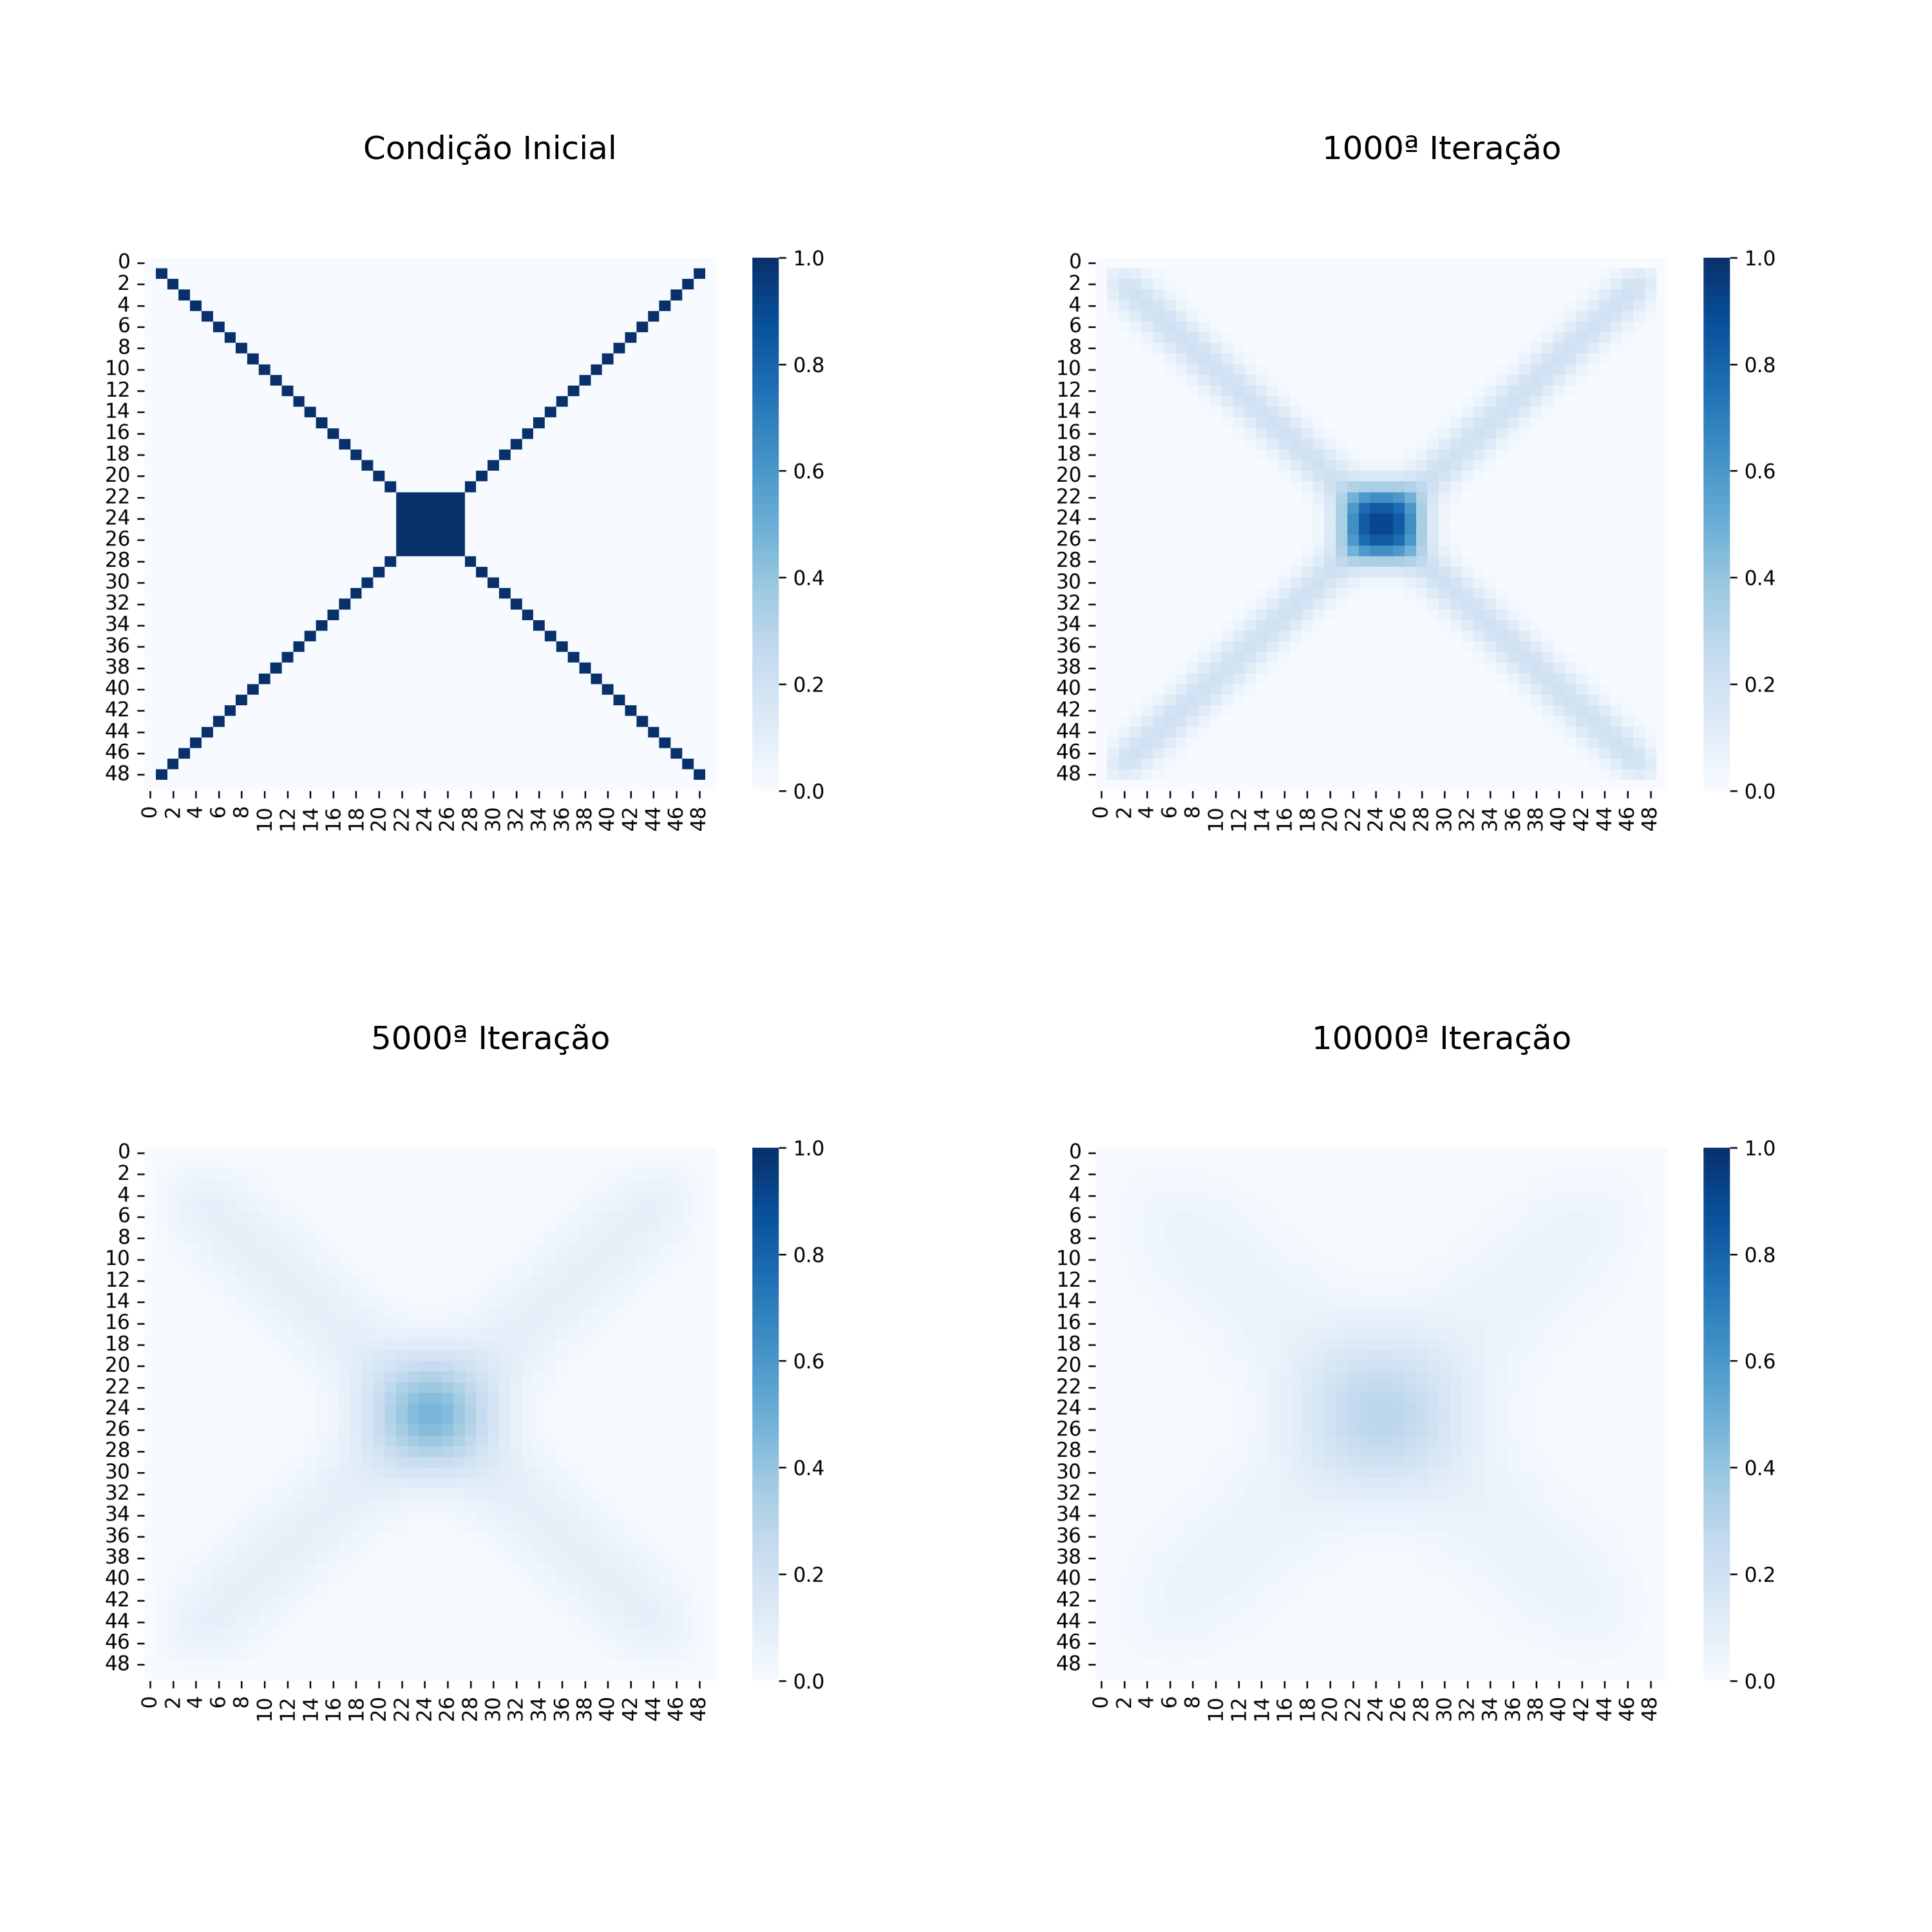
\includegraphics[width=.5\textwidth]{figs/heatmap.png}
  \caption{Mapa de calor em quatro instantes distintos da simulação.}\label{fig:heatmap}
\end{figure}

Analisando a progressão dos mapas de calor, observamos que o comportamento faz
sentido no contexto da solução proposta. Inicialmente, o contaminante é
adicionado com alta concentração nas diagonais e no centro da matriz,
evidenciado pelas regiões azuis-escuros. Com o avanço das iterações, o
contaminante começa a se difundir para as regiões adjacentes, aumentando
gradativamente a luminosidade nessas áreas e diminuindo nos pontos de
concentração inicial. Na última iteração, a concentração se distribui
uniformemente pela matriz, com valores próximos entre si.

\subsection{Análise de Desempenho}

A análise de desempenho foi realizada em um computador \textit{desktop} com as
especificações apresentadas na Tabela~\ref{tab:especificacaoHardware}. Ademais,
as especificações dos parâmetros do problema foram incluídas na
Tabela~\ref{tab:especificacaoSimulacao}.

\begin{table}[ht]
  \centering
  \caption{Tabela de especificação de Hardware}
  \vspace{0.3cm}
  \begin{tabular}{||c c||}
    \hline
    Especificações      & Detalhes                         \\ [0.5ex]
    \hline\hline
    Processador         & Intel i7--7500U @ 2.7GHz--3.5GHz \\
    \hline
    Núcleos / Lógicos   & 2 / 4                            \\
    \hline
    Memória RAM         & 10 GB                            \\
    \hline
    Sistema Operacional & Ubuntu 22.04.05 (via WSL)        \\
    \hline
  \end{tabular}\label{tab:especificacaoHardware}
\end{table}

\begin{table}[ht]
  \centering
  \caption{Tabela de especificação da Simulação}
  \vspace{0.3cm}
  \begin{tabular}{||c c||}
    \hline
    Especificações             & Detalhes                    \\ [0.5ex]
    \hline\hline
    Dimensão da Matriz (N x N) & 3000 x 3000                 \\
    \hline
    Número de Iterações        & 1000                        \\
    \hline
    Distribuição Inicial       & Alta concentração no centro \\
    \hline
    Coeficiente de Difusão     & 0.1                         \\
    \hline
    $\Delta t$                 & 0.01                        \\
    \hline
    $\Delta x$                 & 1.0                         \\
    \hline
  \end{tabular}\label{tab:especificacaoSimulacao}
\end{table}

Para obter valores mais consistentes e minimizar influências externas, como
outros programas em execução, cada teste foi executado quinze vezes e, assim,
calculamos o tempo médio gasto e seu desvio padrão. O \textit{speedup} é
calculado dividindo-se o tempo de execução sequencial pelo tempo de execução
CUDA correspondente.

\begin{table}[ht]
  \centering
  \caption{Tabela de comparação de desempenho entre o código sequencial e o
    utilizando CUDA.}\label{tab:Resultados}
  \vspace{0.3cm}
  \begin{tabular}{||c c c c||}
    \hline
    Experimento     & N°Threads & Tempo             & SpeedUp \\ [0.5ex]
    \hline\hline
    Sequencial      & 1.0       & 124.10 $\pm$ 3.86 & 1.0     \\
    \hline
    OMP (4 Threads) & -         & - $\pm$ -         & -       \\
    \hline
    CUDA(16, 16)    & 9078169.0 & 23.32 $\pm$ 0.52  & 5.32    \\
    \hline
    CUDA(32, 32)    & 9174841.0 & 25.05 $\pm$ 0.49  & 4.95    \\
    \hline
  \end{tabular}
\end{table}

\begin{figure}[ht]
  \centering
  \begin{minipage}[b]{0.45\textwidth}
    \centering
    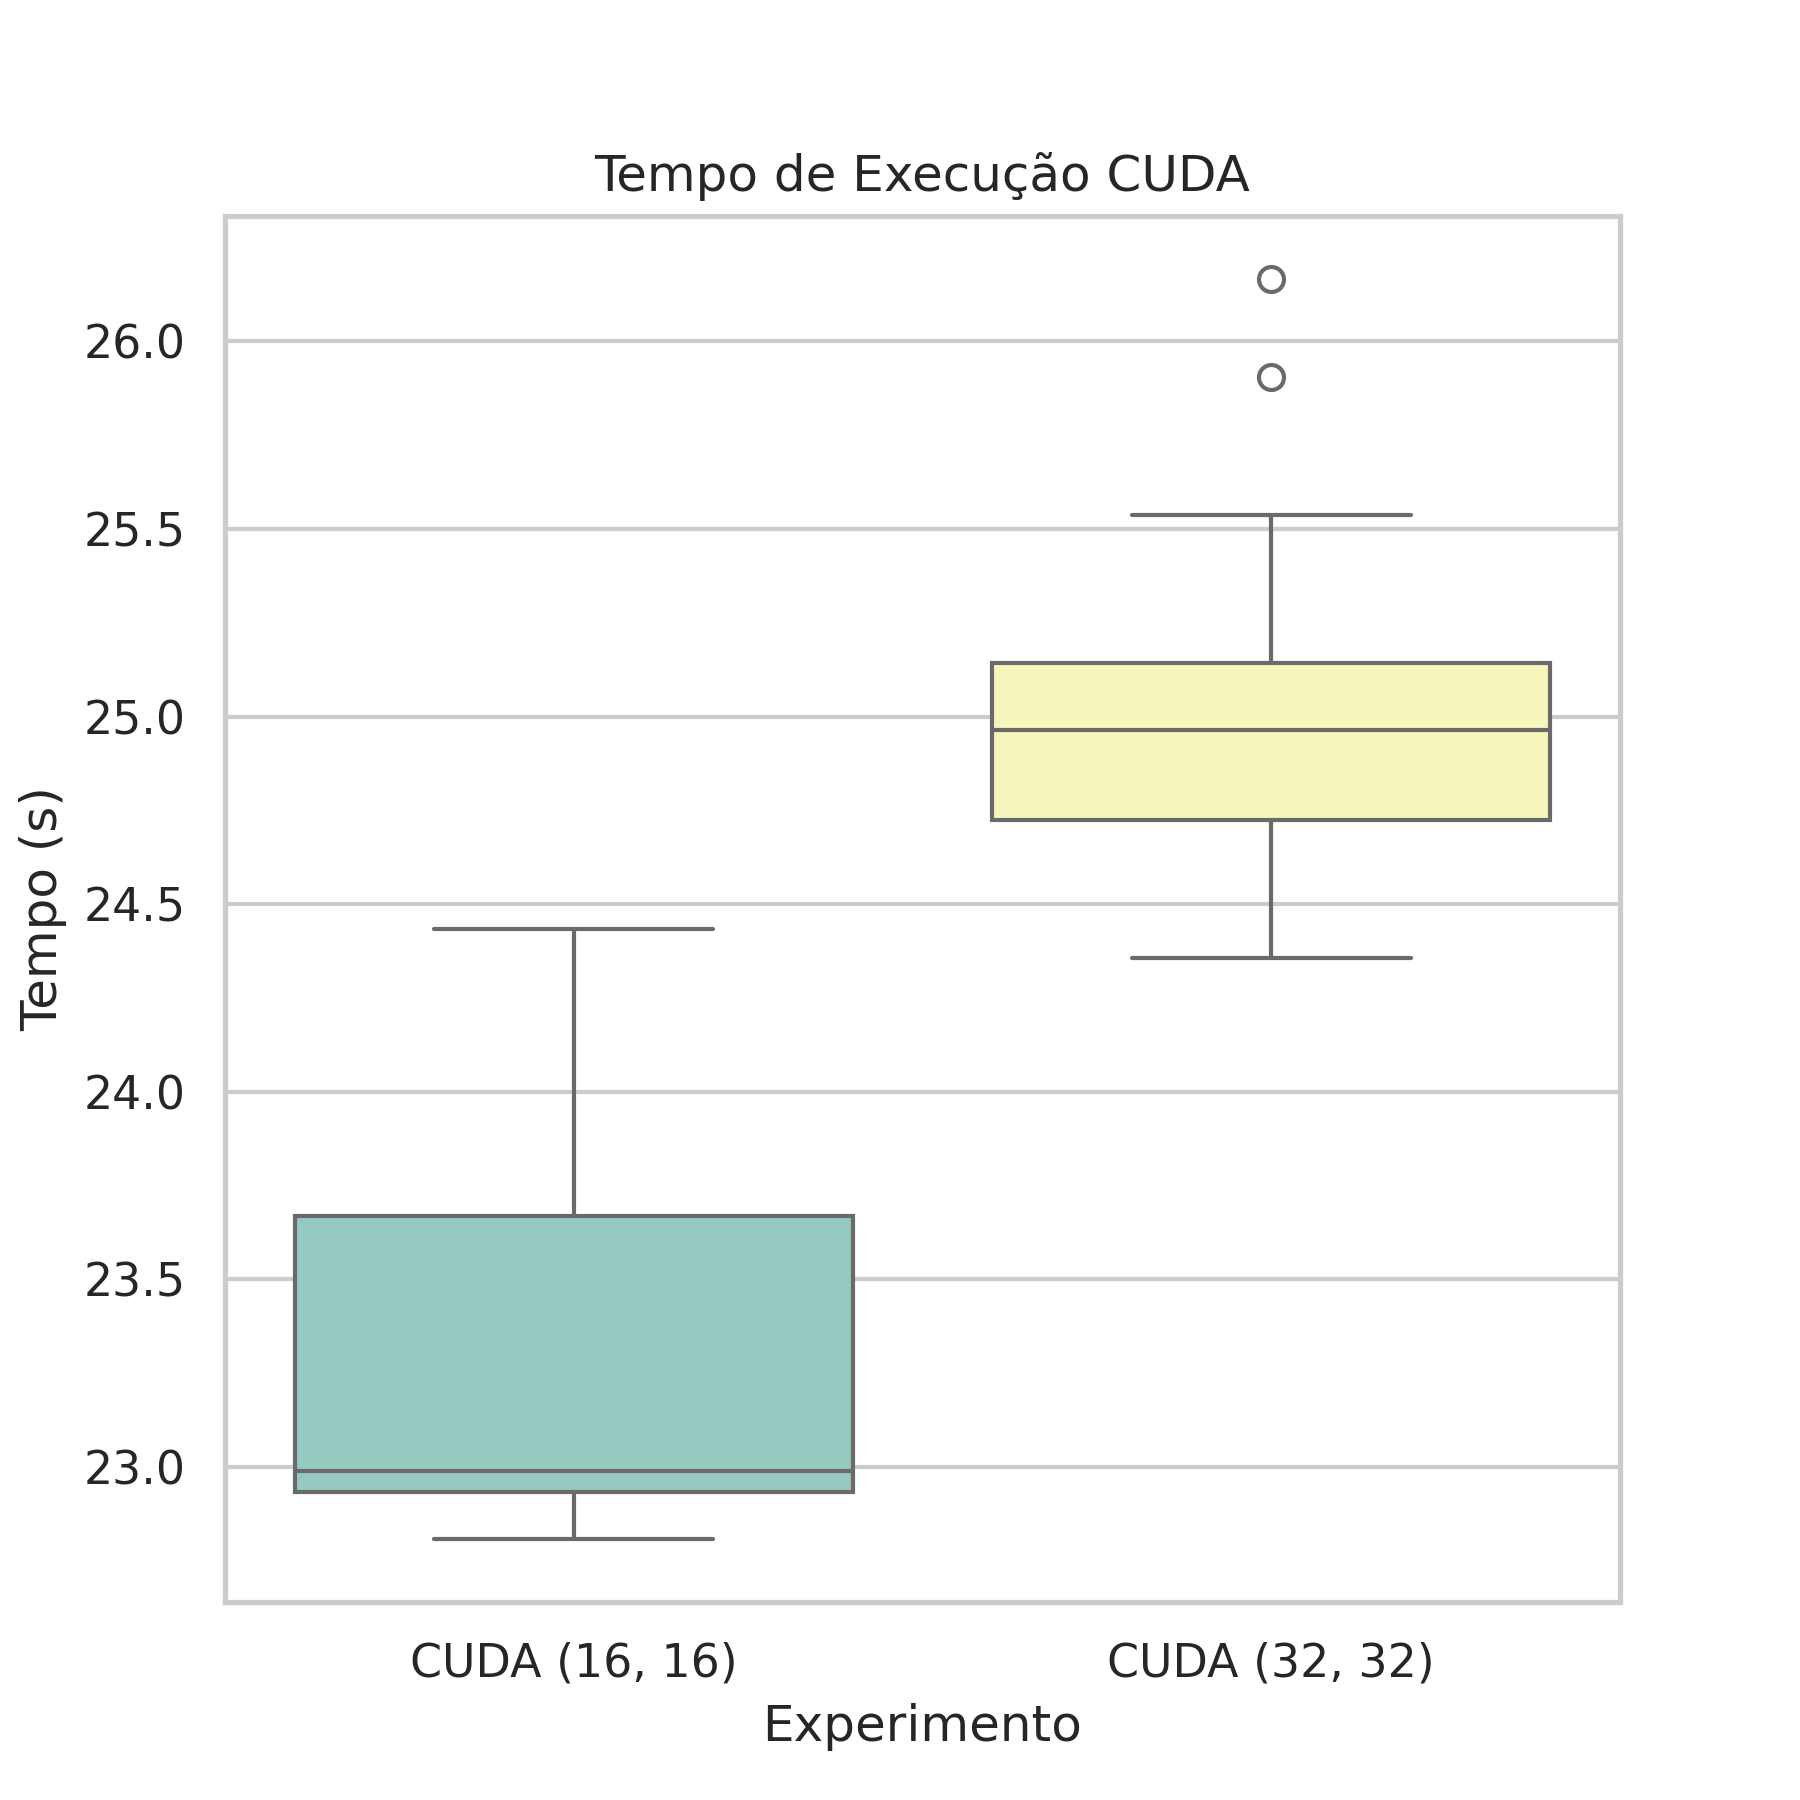
\includegraphics[width=\textwidth]{figs/times_boxplot_cuda.png}
  \end{minipage}
  \begin{minipage}[b]{0.3\textwidth}
    \centering
    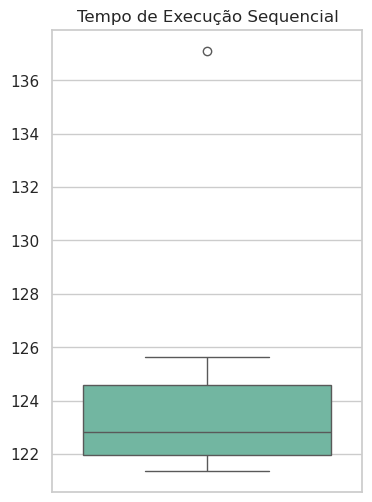
\includegraphics[width=\textwidth]{figs/times_boxplot_sequential.png}
  \end{minipage}
  \caption{Gráficos \textit{boxplots} para os tempos de execução medidos para cada um dos experimentos registrados na Tabela~\ref{tab:Resultados}. }\label{fig:Boxplots}
\end{figure}

A visualização dos dados por meio de gráficos de \textit{boxplot}
(Figura~\ref{fig:Boxplots}) é um ótimo meio para avaliar o desempenho do
algoritmo, considerando as possíveis incertezas que advêm do sistema
computacional em que ele está inserido. Problemas de priorização de tarefas,
alocação de recursos e utilização do sistema pelo usuário podem introduzir
variações significativas no tempo de execução e na eficiência geral do
algoritmo. Essas flutuações são facilmente identificadas por meio dos gráficos,
ilustrando que existe uma pequena diferença de poucos segundos que podem
influenciar no tempo de execução final do programa.

Nota-se uma grande eficiência do tempo de execução do algoritmo de CUDA em
relação ao sequencial e OpenMP, o que demonstra o quão importante esse hardware
pode ser para tarefas que demandam cálculos extremos, como os de aprendizado de
máquina, por exemplo. Porém, importante ressaltar que esse ganho será menor se
o tamanho da simulação for reduzido, já que todo o processo de alocar, enviar e
receber dados e administrar a GPU possui um custo, que pode ser evitado ao
utilizar apenas as threads da própria CPU.

O desempenho inferior do CUDA com \textit{block dim} (32, 32) em relação ao
(16, 16) ocorre porque blocos maiores podem causar um maior uso de recursos,
como memória compartilhada e registradores, levando à saturação da capacidade
da GPU. Isso resulta em maior latência devido à competição entre blocos por
recursos limitados.

\section{Conclusão}

Com a introdução da implementação paralela utilizando CUDA, além da sequência e
da versão OpenMP previamente analisadas, validou-se a correção dos resultados
ao longo das diferentes abordagens e examinou-se o impacto do paralelismo no
tempo de execução. Os experimentos demonstraram que, embora a paralelização com
CUDA proporcione ganhos significativos em relação ao código sequencial, podem
existir limitações na escalabilidade, que são decorrentes de \textit{overheads}
de comunicação entre a CPU e a GPU, latências de memória e restrições
arquiteturais do próprio hardware gráfico.

Dessa forma, o estudo evidencia não apenas as vantagens práticas da
paralelização em termos de desempenho e eficiência em simulações numéricas, mas
também ressalta a importância de se compreender os desafios inerentes às
diferentes estratégias paralelas. A experiência com CUDA complementa os
conceitos fundamentais aprendidos em programação concorrente e distribuída,
oferecendo percepções valiosas sobre a aplicabilidade e os limites da
aceleração por GPU em contextos computacionais exigentes.

\bibliographystyle{sbc}
\bibliography{sbc-template}
\nocite{*}
\end{document}